% NOTES:
%%    do we want to explore for larger S?  Does false positive rate change?

% review: first round, chris, enbody, cole/jordan?
% second round yanni, curt, james foster, abdol.

% TEST

\documentclass[12pt]{article} \usepackage{simplemargins}
\usepackage[pdftex]{graphicx} \graphicspath{{figures/}}

\setlength{\parindent}{0pt} \setlength{\parskip}{1.6ex}
\setallmargins{1in} \linespread{1.6}

\begin{document}

\title{A probabilistic framework for compressible assembly graphs}
\author{Jason Pell, Arend Hintze, Rosangela Canino-Koning, C. Titus Brown}

\maketitle

\section{Abstract}

The memory requirements for de novo assembly of shotgun sequencing
data from metagenome and transcriptome samples are an increasingly
large practical barrier to next-generation sequence analysis.  Here we
introduce a novel probabilistic graph representation for de Bruijn
graphs that is based on Bloom filters.  This representation is
extremely memory efficient, enabling storage of de Bruijn graphs with
6 bits per node.  While the graph contains false nodes and
edges due to the underlying probabilistic representation, we show that
it can be used to assess global graph structure with high accuracy
until a specific false positive rate is reached.  We demonstrate the
utility of this representation for graph partitioning, an approach
that decomposes de Bruijn graphs into disconnected components in order
to decrease memory and compute requirements for sequence assembly.

%% @@CTB do we show 6 bits/node??

\section{Introduction}

De novo assembly of shotgun sequencing data sets is extremely memory
intensive, and it is now easy to generate more sequencing data than
can be handled on commodity computing hardware.  This is especially
true in metagenomics, where assembling shotgun sequences
from complex microbial samples required 512 GB or more of RAM
(MetaHit, rumen).  Assembling transcriptome data from non-model
organisms also requires substantial amounts of memory, e.g. 1 GB of
RAM per million reads (Trinity).  These substantial memory requirements for
assembling large data sets are increasingly becoming an obstacle to
sequence analysis in metagenomics and transcriptomics (refs).

The predominant assembly formalism applied to short-read sequencing
data sets from Illumina, SOLiD, and Roche 454 machines is a de Bruijn
graph.  In a de Bruijn graph approach, sequencing reads are decomposed
into fixed-length words, or k-mers, and used to build a connectivity
graph.  This graph is then traversed to determine contiguous sequences
made from overlapping k-mers.  Because de Bruijn graphs store only
k-mers, memory usage scales with the number of unique k-mers in the
data set rather than the number of reads.  Thus human genomes can be
assembled in as little as 512 GB or RAM(ref ALLPATHS-LG).  For
more complex samples such as soil metagenomes, which may possess a
million or more species, terabytes of memory are required to store the
graph.  With mRNA samples that require deep sequencing to sample rare
molecules, novel k-mers introduced by sequencing error may result in
similarly large memory requirements.

One approach to de novo assembly of metagenomes and transcriptomes is
to apply graph partitioning, in which the de Bruijn graph is divided
up into largely disconnected components (Trinity, metaIDB,
MetaVelvet).  While the initial partitioning step is as memory
intensive as assembly, once the graph is partitioned the components
can be assembled individually with parameters chosen for each
component (cite).  This results in improved assemblies, but does not
address memory scaling.

To apply partitioning to memory scaling , we here describe a novel
probabilistic representation for storing de Bruijn graphs in memory,
based on Bloom filters (citations).  Bloom filters are constant-memory
probabilistic data structures for storing sets; essentially hash
tables without collision detection, they can yield false positives on
set membership queries, but not false negatives.  We show that this
probabilistic graph representation can be used to efficiently store
and traverse DNA de Bruijn graphs with an approximately 20-fold
decrease in memory usage over the Velvet assembler. Moreover, this
graph representation can be used to accurately partition assembly
graphs.  We relate changes in local and global garph connectivity
to the false positive rate of the underlying Bloom filters, and
show that the graph's global structure is accurate until an abrupt
transition in false connectivity near a false positive rate of 0.183,
corresponding to a lower memory limit of 6 bits per graph node.

% @@ figure for how we're storing DBGs in a Bloom filter.
% @@ push ecoli % to 15% memory
% @@ exact/inexact data influence

\section{Methods}

\subsection{Genome and Sequence Data}
We used \emph{E. coli} K-12 MG1655 genome (GenBank: U00096.2) and two MG1655 Illumina 
datasets (Short Read Archive accessions SRR074860 and SRR074861). 

\subsection{Data Structure Implementation}
% @JAP I added and merged some stuff, but I think the language needs to be 
% more ``direct''
We implemented a variation on the Bloom filter data structure to store
k-mers in memory. In a classic Bloom filter, multiple hash functions
map into a single hash table to add an object or test for the presence
of an object in the set. In our variant, we use multiple
prime-number-sized hash tables with each having a different hash
function corresponding to the modulus of the DNA bitstring
representation with the hash table size; the underlying properties of
the Bloom filter are identical, however.  To add a k-mer to the
filter, the corresponding bit is set to 1 in each hash table.  To find
the presence of a k-mer, each table is queried for the presence of
that k-mer; for a k-mer to be considered present in the dataset, the
k-mer must be found in all of the hash tables.  If a k-mer is not
present in any one hash table, then it is certainly not in the
dataset. As a result, there is a one-sided error: false positives are
possible but false negatives are not. The expected false positive rate
is simply the product of the occupancies of the hash tables.  As with
other hash-style data structures, Bloom filters have a fast lookup
time, $O(h)$ for $h$ hash tables.  Similar to other hash-style data
structures for storing k-mers, memory usage is independent of the
value of $k$.

\subsection{Calculating Data Structure Properties}
The properties of our Bloom filter variant are essentially the
same as a classical Bloom filter \cite{bloomsurvey}.
For example, to calculate the expected false positive 
rate, we
take the product of the occupancy of each hash table:
\begin{displaymath}
P_f = \prod_{h \in H} occ(h)
\end{displaymath}
where $h$ is a hash table in the set of hash tables $H$ and $occ$ denotes
the occupancy (proportion of bits set) for a hash table.
We can find the optimal number of hash tables
to use by calculating
\begin{displaymath}
\vert H \vert_{opt} = \ln 2 \frac{m}{k}
\end{displaymath}
where $m$ is the amount of memory in bits to allocate and $k$
is the number of unique k-mers to be inserted. Finally,
the number of bits per
k-mer used in the data structure for the optimal number of hash 
tables is

\begin{displaymath}
\frac{m}{n} = \frac{1}{\ln(2)} \log{\frac{1}{P_f}}.
\end{displaymath}

\subsection{Using The Bloom Filter As A K-mer Graph}
% @CTB FIGURE
Having stored the k-mers in a Bloom filter, we can traverse
the data as a k-mer graph. We let each k-mer be a vertex, where
the reverse complement of a k-mer is considered the same
vertex. Each k-mer can
have up to eight neighbors, which are any of the other k-mers that
 share a $k-1$
overlap; no explicit edge is stored. In doing so, we implicitly 
treat the graph as a simple graph as opposed to a multigraph or 
digraph, which means that there can be no self-loops or parallel 
edges between vertices/k-mers. This graph representation is constant 
in its memory usage, so only ancillary information such as list 
of vertices visited or waypoints in the graph consumes additional 
memory.

This graph structure is effectively {\em compressible}
because one can choose a larger
or smaller size for the underlying Bloom filters; a larger size admits fewer
false positives, while a smaller size admits more. By relying on Bloom
filters, the data structure is constant memory: no extra memory is
used as additional data is added. However, as memory is decreased or data
is increased, only false positive vertices and edges are gained, so
compressing the graph results in a more tightly interconnected graph.

In contrast to an exact approach, there is a chance that a k-mer 
will be adjacent to a false positive,
that is, a k-mer
that does not actually exist in the original dataset but registers as present  
due to 
the Bloom filter. If this probability is too high, the 
graph can become dominated by false connectivity. 
Intuitively, it is clear that when most real k-mers
have at least one erroneous neighbor ($p_f \approx \frac{1}{8}$), 
false paths between real (but unconnected) k-mers are likely to 
appear. However, it is not immediately clear at exactly what 
false positive rate this occurs. We address this below.  % clumsy, I know.

\subsection{Estimating False Positive Rate For Erroneous Connectivity}
We ran a simulation to find when connected components in the graph 
begin to erroneously connect to one another.
To calculate the false positive rate $p$ at which this aberrant 
connectivity occurs, 
we added random k-mers, sampled from a uniform GC distribution, to the data structure 
and then calculated the occupancy and size of 
the largest connected 
component. From this we sampled the relative size of 
the largest component and the overall cluster size distribution for each
given occupancy rate.
At the occupancy where a ``giant cluster'' appears, this cluster size distribution 
must be scale-free \cite{stauffer1979scaling}. 

We then found at what value of $p$ the resulting 
cluster size distribution in logarithmic 
scale can be better fitted in a linear or quadratic fashion using 
the F-statistic
\newline
\newline
\begin{displaymath}
F=\frac{RSS_1-RSS_2}{p_2-p_1} \times \frac{n - p_2}{RSS_2}
\end{displaymath}
% @CTB DEFINE RSS, p, n

where $RSS_i$ is the residual sum of squares for model $i$, $p_i$ is 
the number of parameters for model $i$, and $n$ is the number of data 
points. To handle the finite size sampling error, the data was binned using the 
threshold binning method \cite{adami2002critical}. The critical value for 
when aberrant connectivity occurred was found by determining the local maxima 
of the F-values.

\subsection{Graph Partitioning Using A Bloom Filter}
We used the Bloom filter data structure containing the k-mers from a
dataset to discover disconnected components of the graph, i.e. to
partition the graph.  Here a connected component is a set of k-mers
whose originating reads overlap transitively by at least $k$ base
pairs.  To partition the reads, we tag the graph at a minimum density
by using the underlying reads as a guide. We then exhaustively explore
the graph around these tags in order to connect tagged k-mers based on
graph connectivity.  The underlying reads in each connected component
can then be separated and analyzed individually without affecting the
overall result, because they do connect outside that read set.

% @CTB mention k_0 > k_1 etc.

\subsection{Software and Software Availability}

We have implemented this compressible graph representation in a
software package named khmer.  It is written in C++ and Python 2.6 and
is available under the BSD open source license at
https://github.com/ctb/khmer.  The graphviz software package was used
for graph visualizations. The scripts to generate the figures of this
paper are available in the khmer repository.

\section{Results}

\subsection{Effect Of False Positives on Local Graph Structure}
We wanted to understand how erroneous neighbors created by false
positives can alter the local graph structure, so we randomly
generated a 1,031bp circular sequence to visualize the effect of false
positives.  After storing this sequence in compressible graphs using
$k=31$ with four different false positive rates ($p_f$=0.01, 0.05,
0.10, and 0.15), we explored the graph using breadth-first search
beginning at the first 31-mer.  The graphs in Figure 1 demonstrate how
the local graph structure elaborates with the false positive rate
while the overall circular graph structure remains, with no erroneous
shortcuts between k-mers that are present in the original
sequence. Because long erroneous paths are unlikely to occur, a
relatively high false positive rate ($\sim$ 15\%) is unlikely to
connect components together erroneously. Note that when the false
positive rate is sufficiently high, the resulting graph is
(practically speaking) impossible to visualize due to the effect of
erroneous k-mers connecting to other erroneous k-mers.

% @CTB I thought percolation threshold was independent of k?  Why does
% large k affect anything??

\begin{figure}
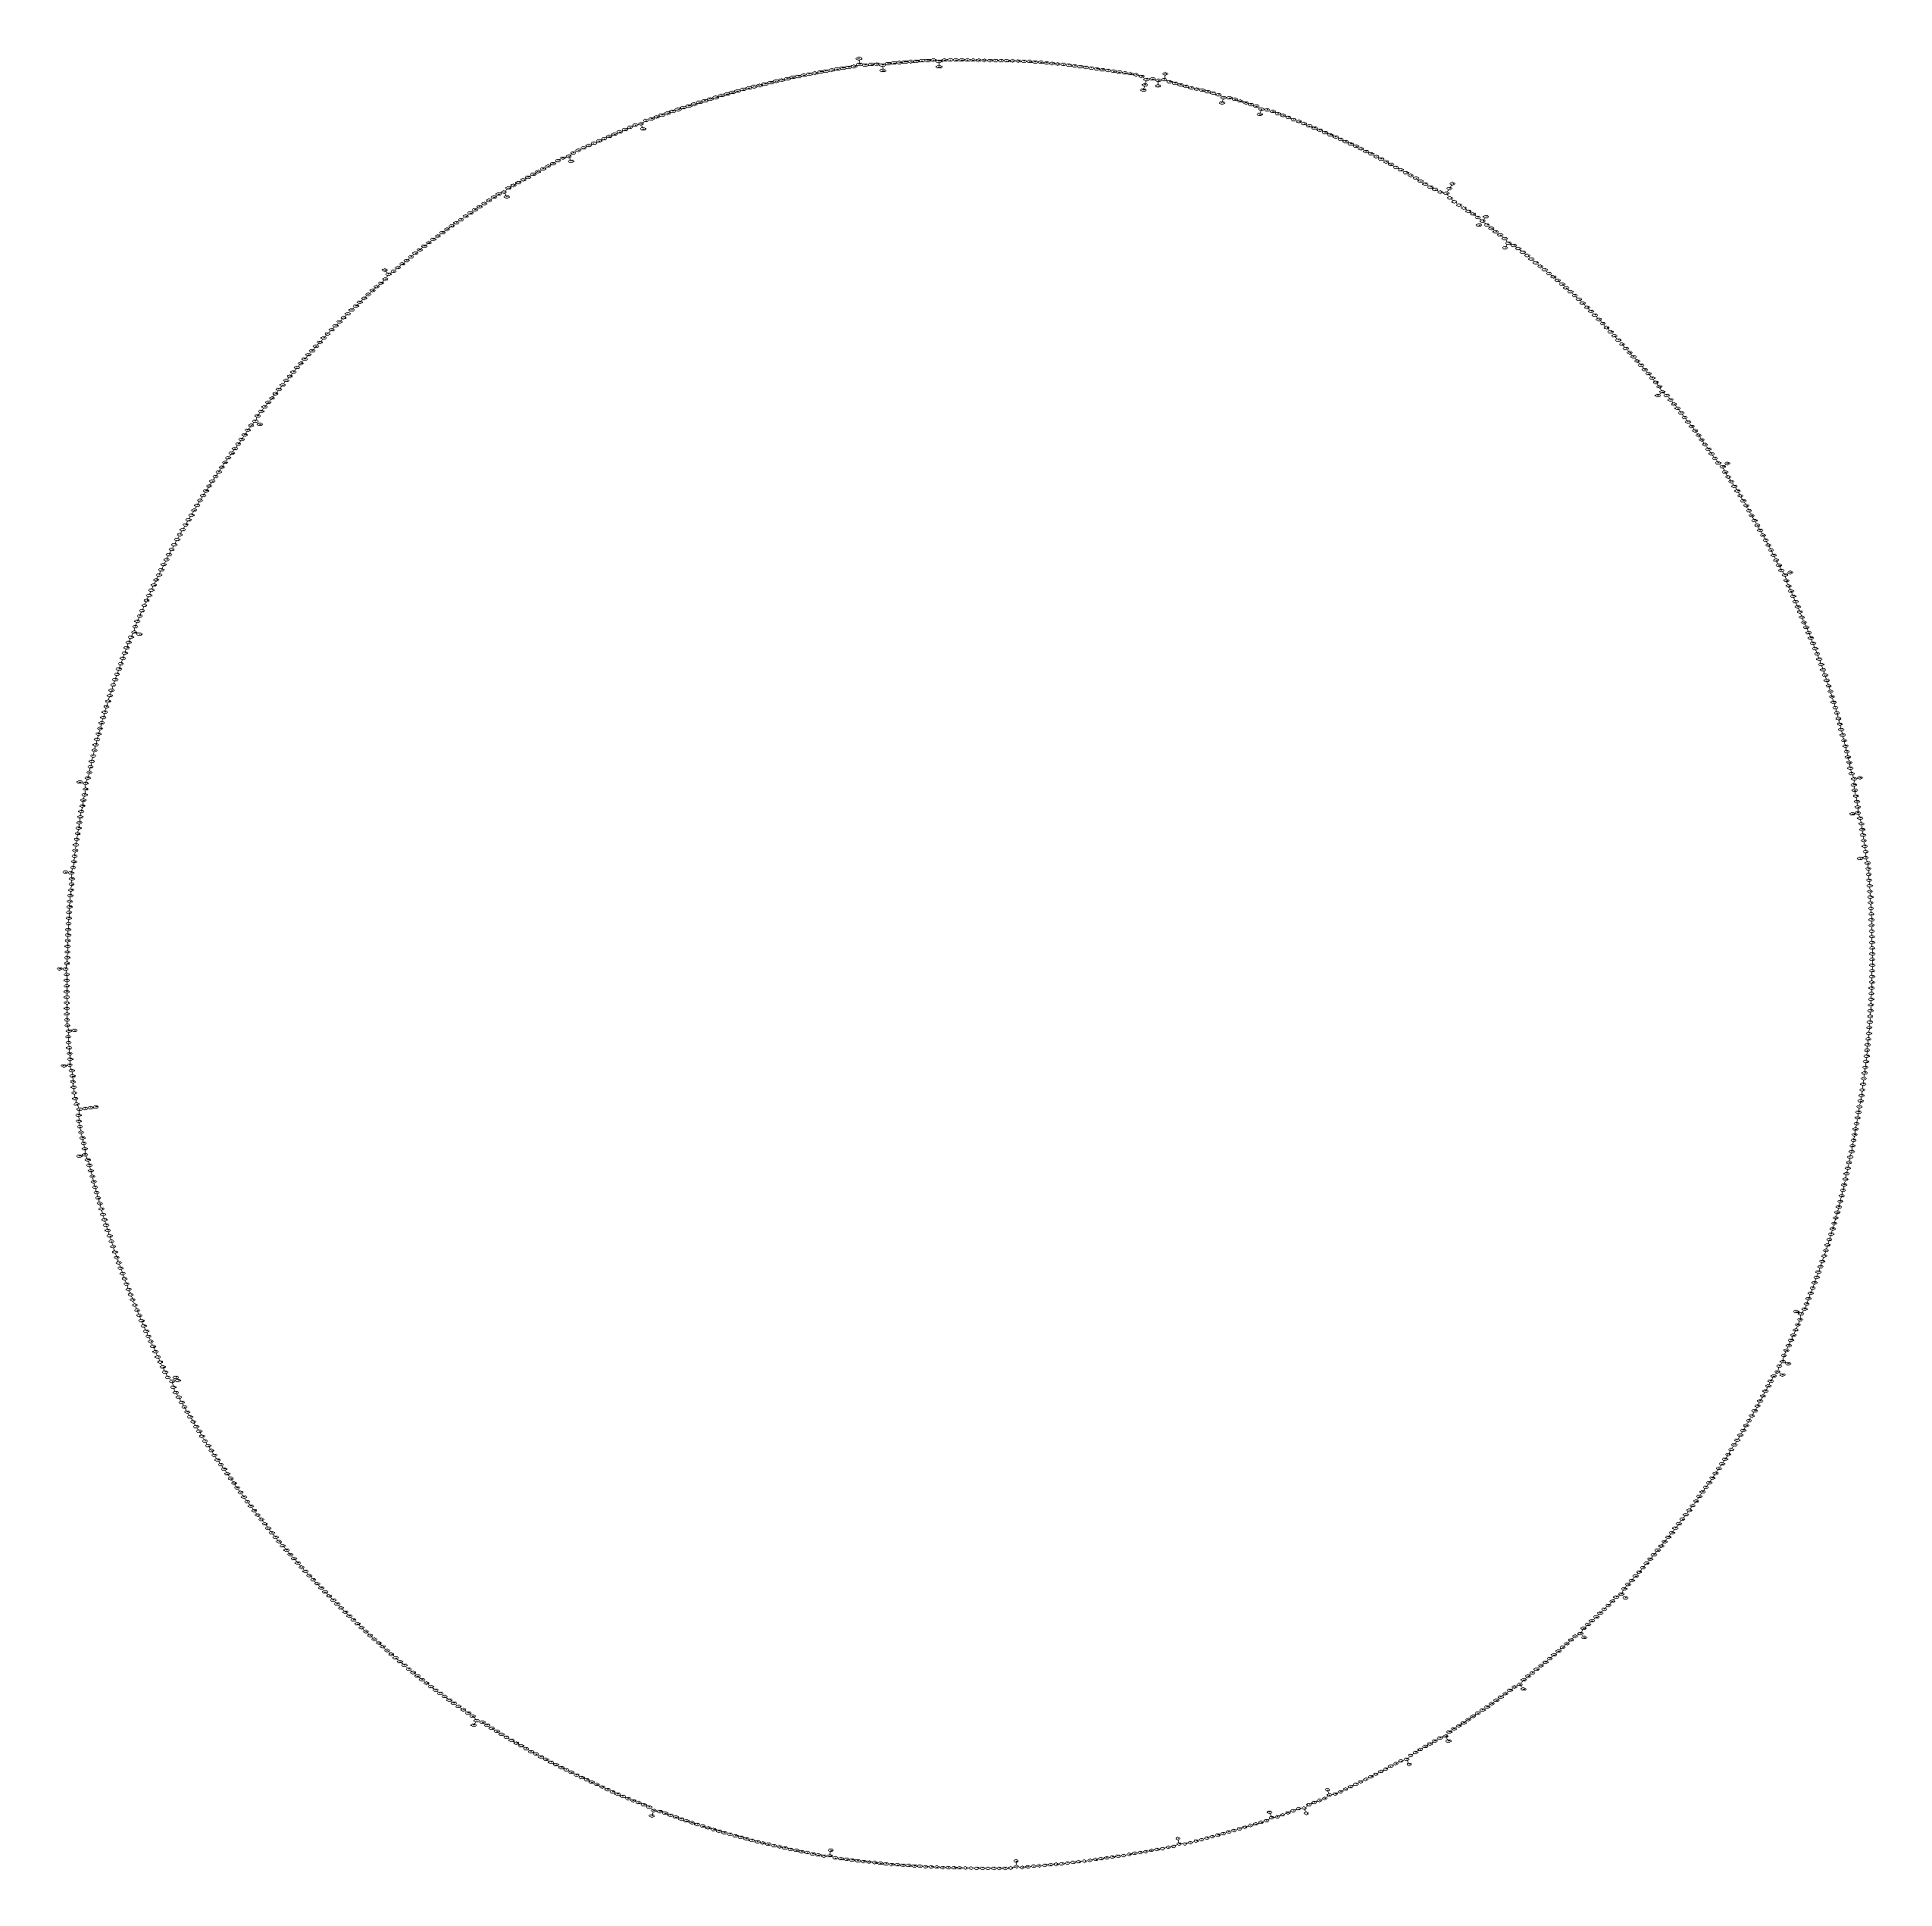
\includegraphics[width=3in]{figures/f3b001}
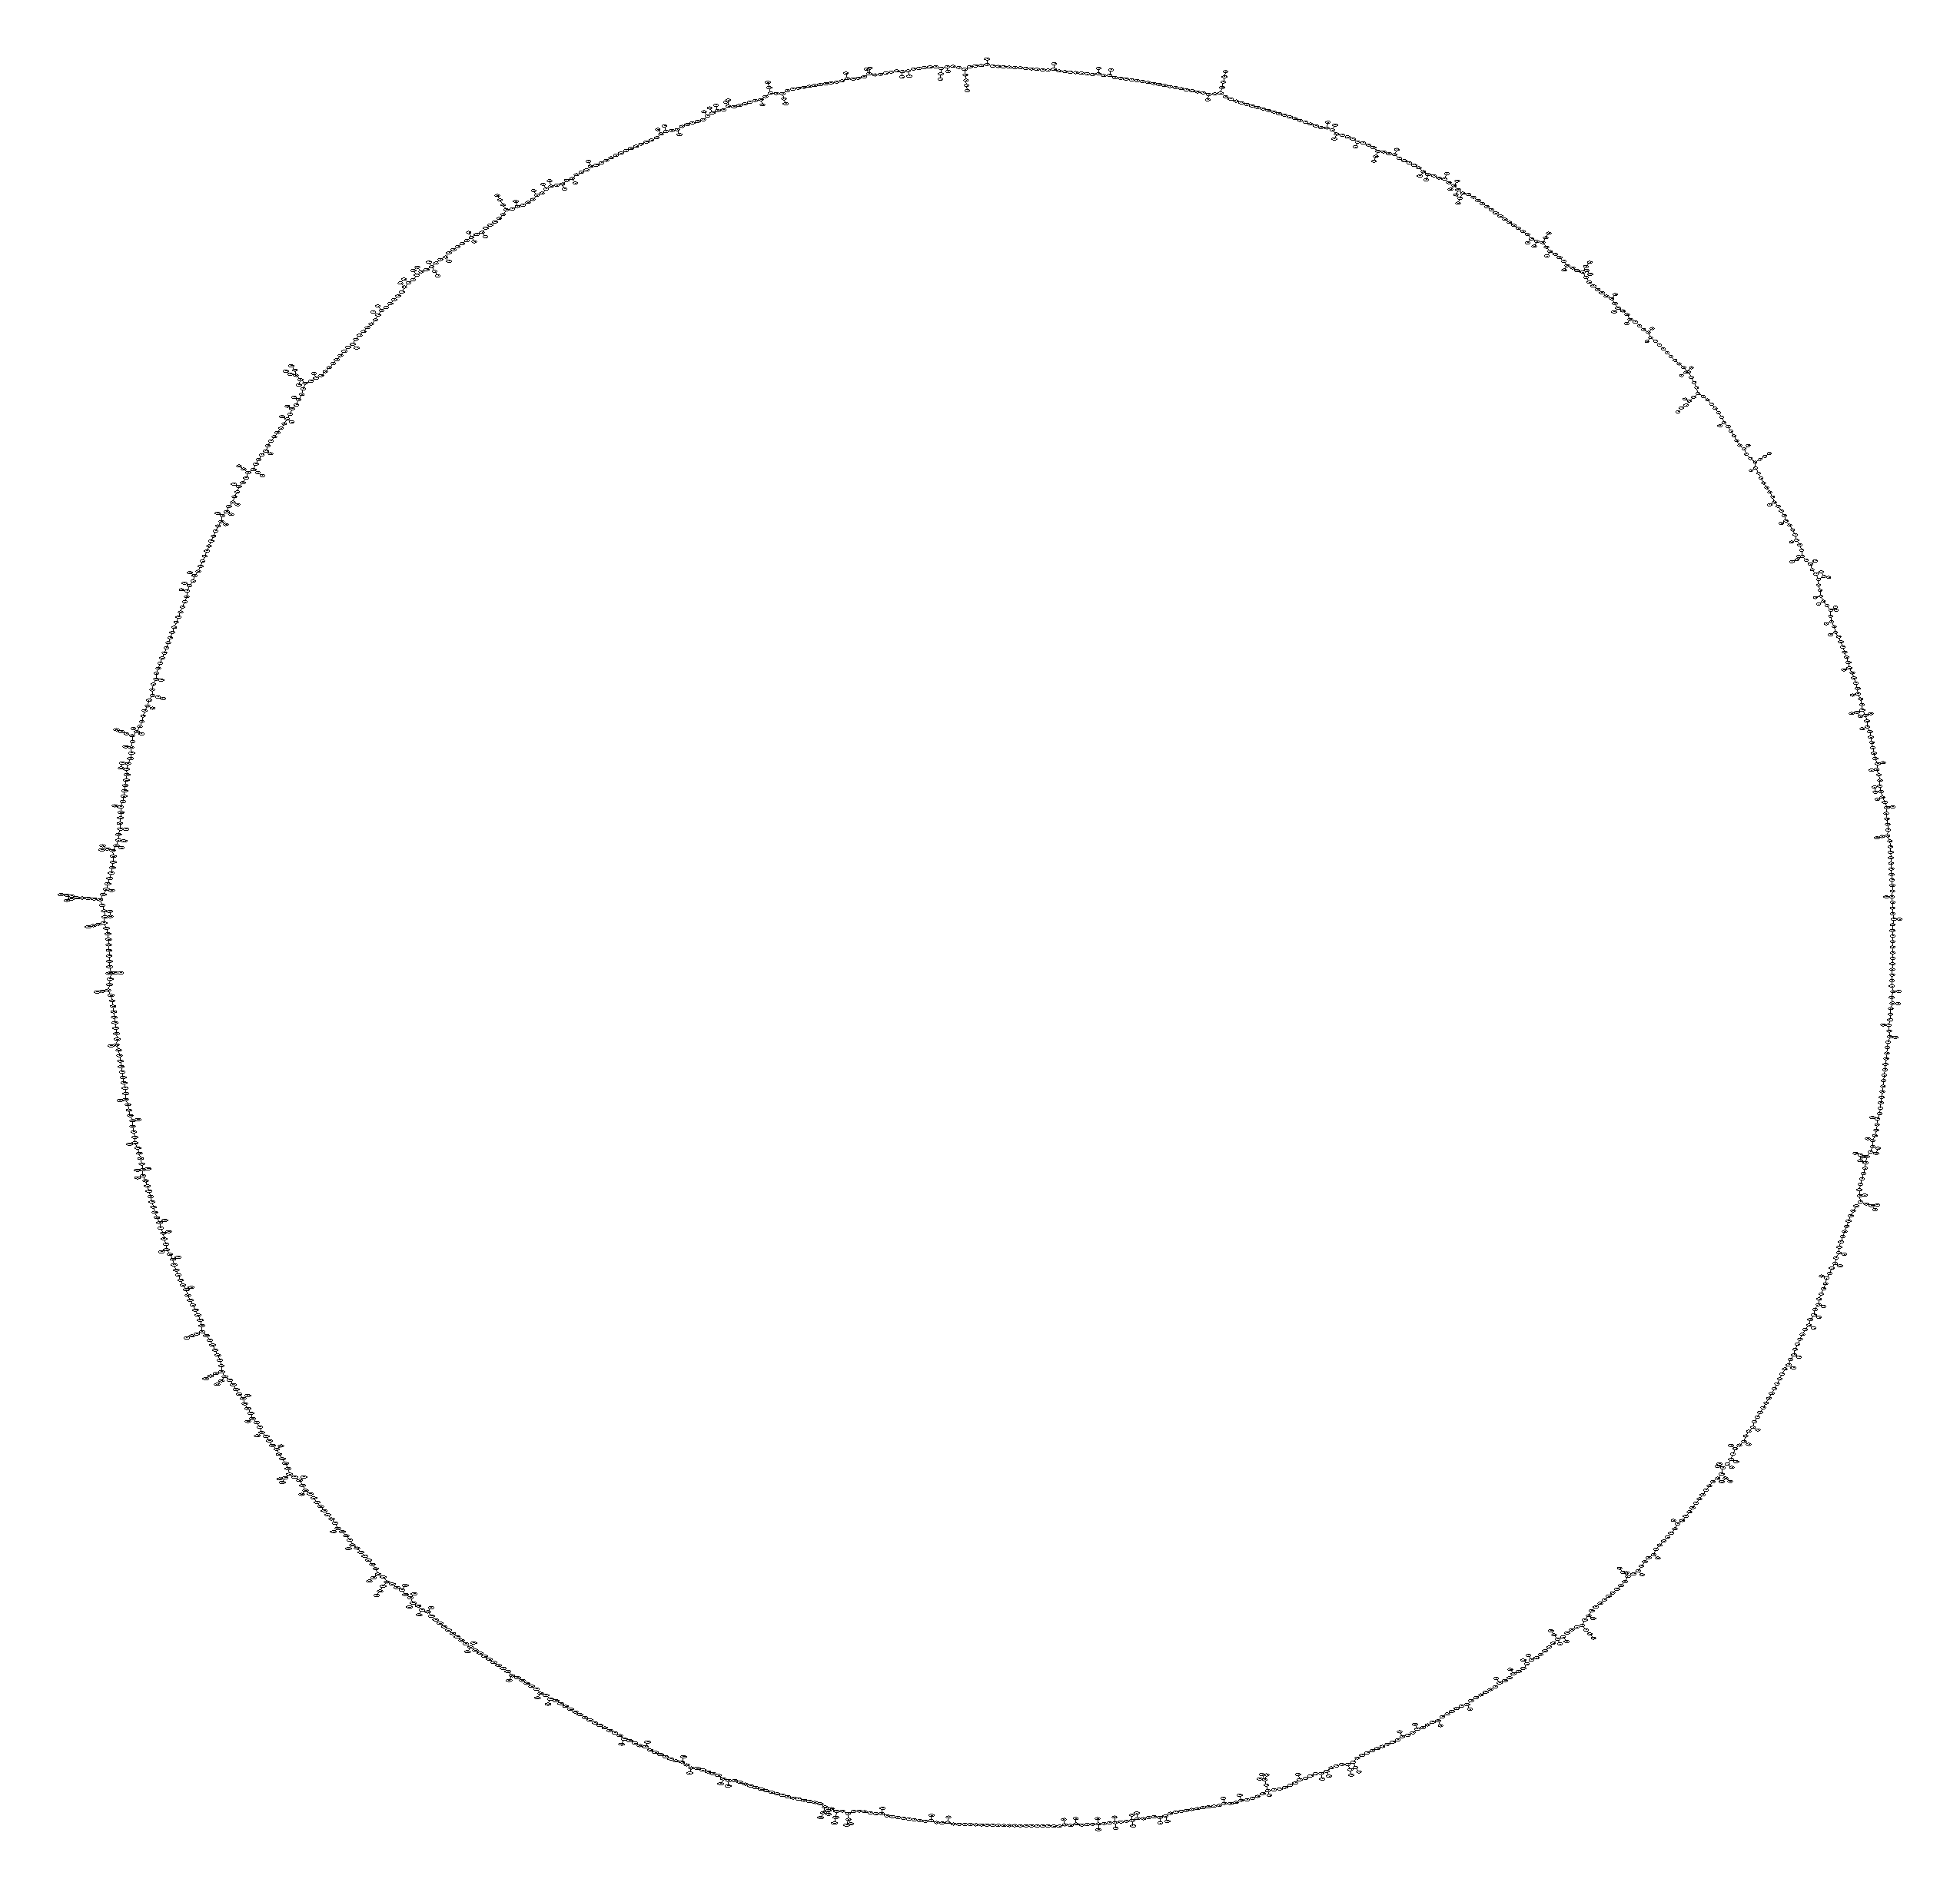
\includegraphics[width=3in]{figures/f3b005}\\
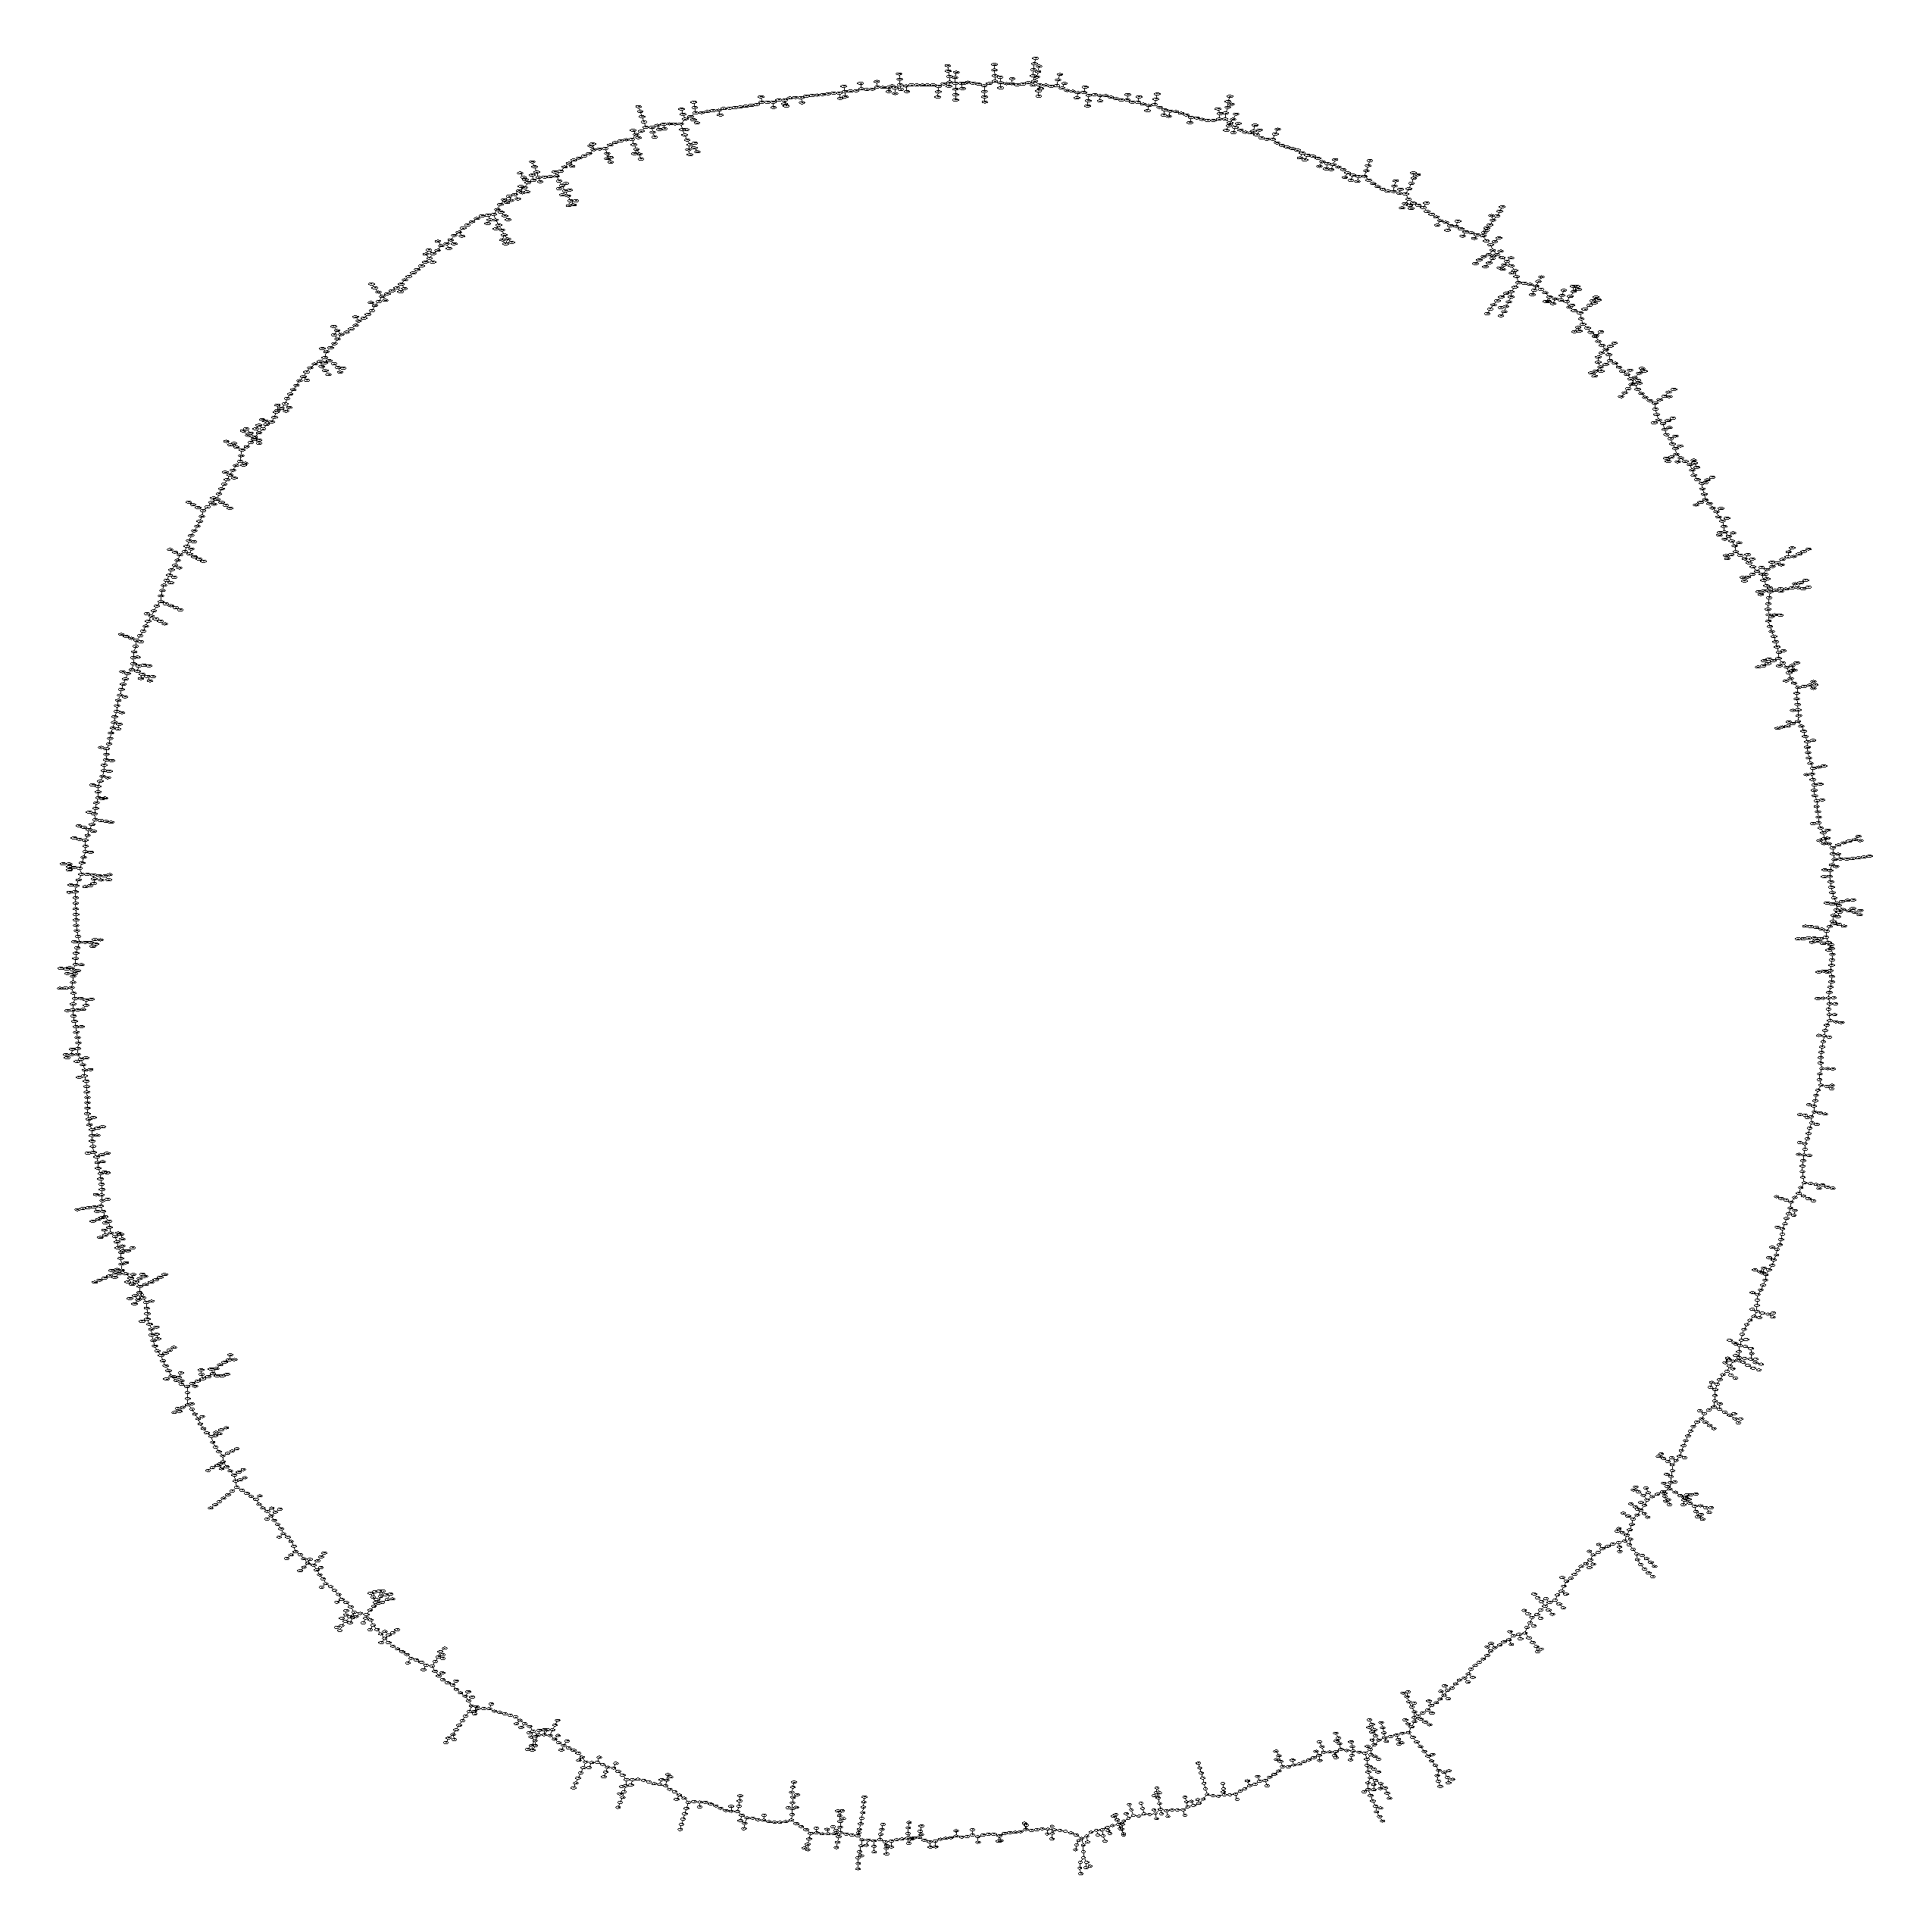
\includegraphics[width=3in]{figures/f3b010}
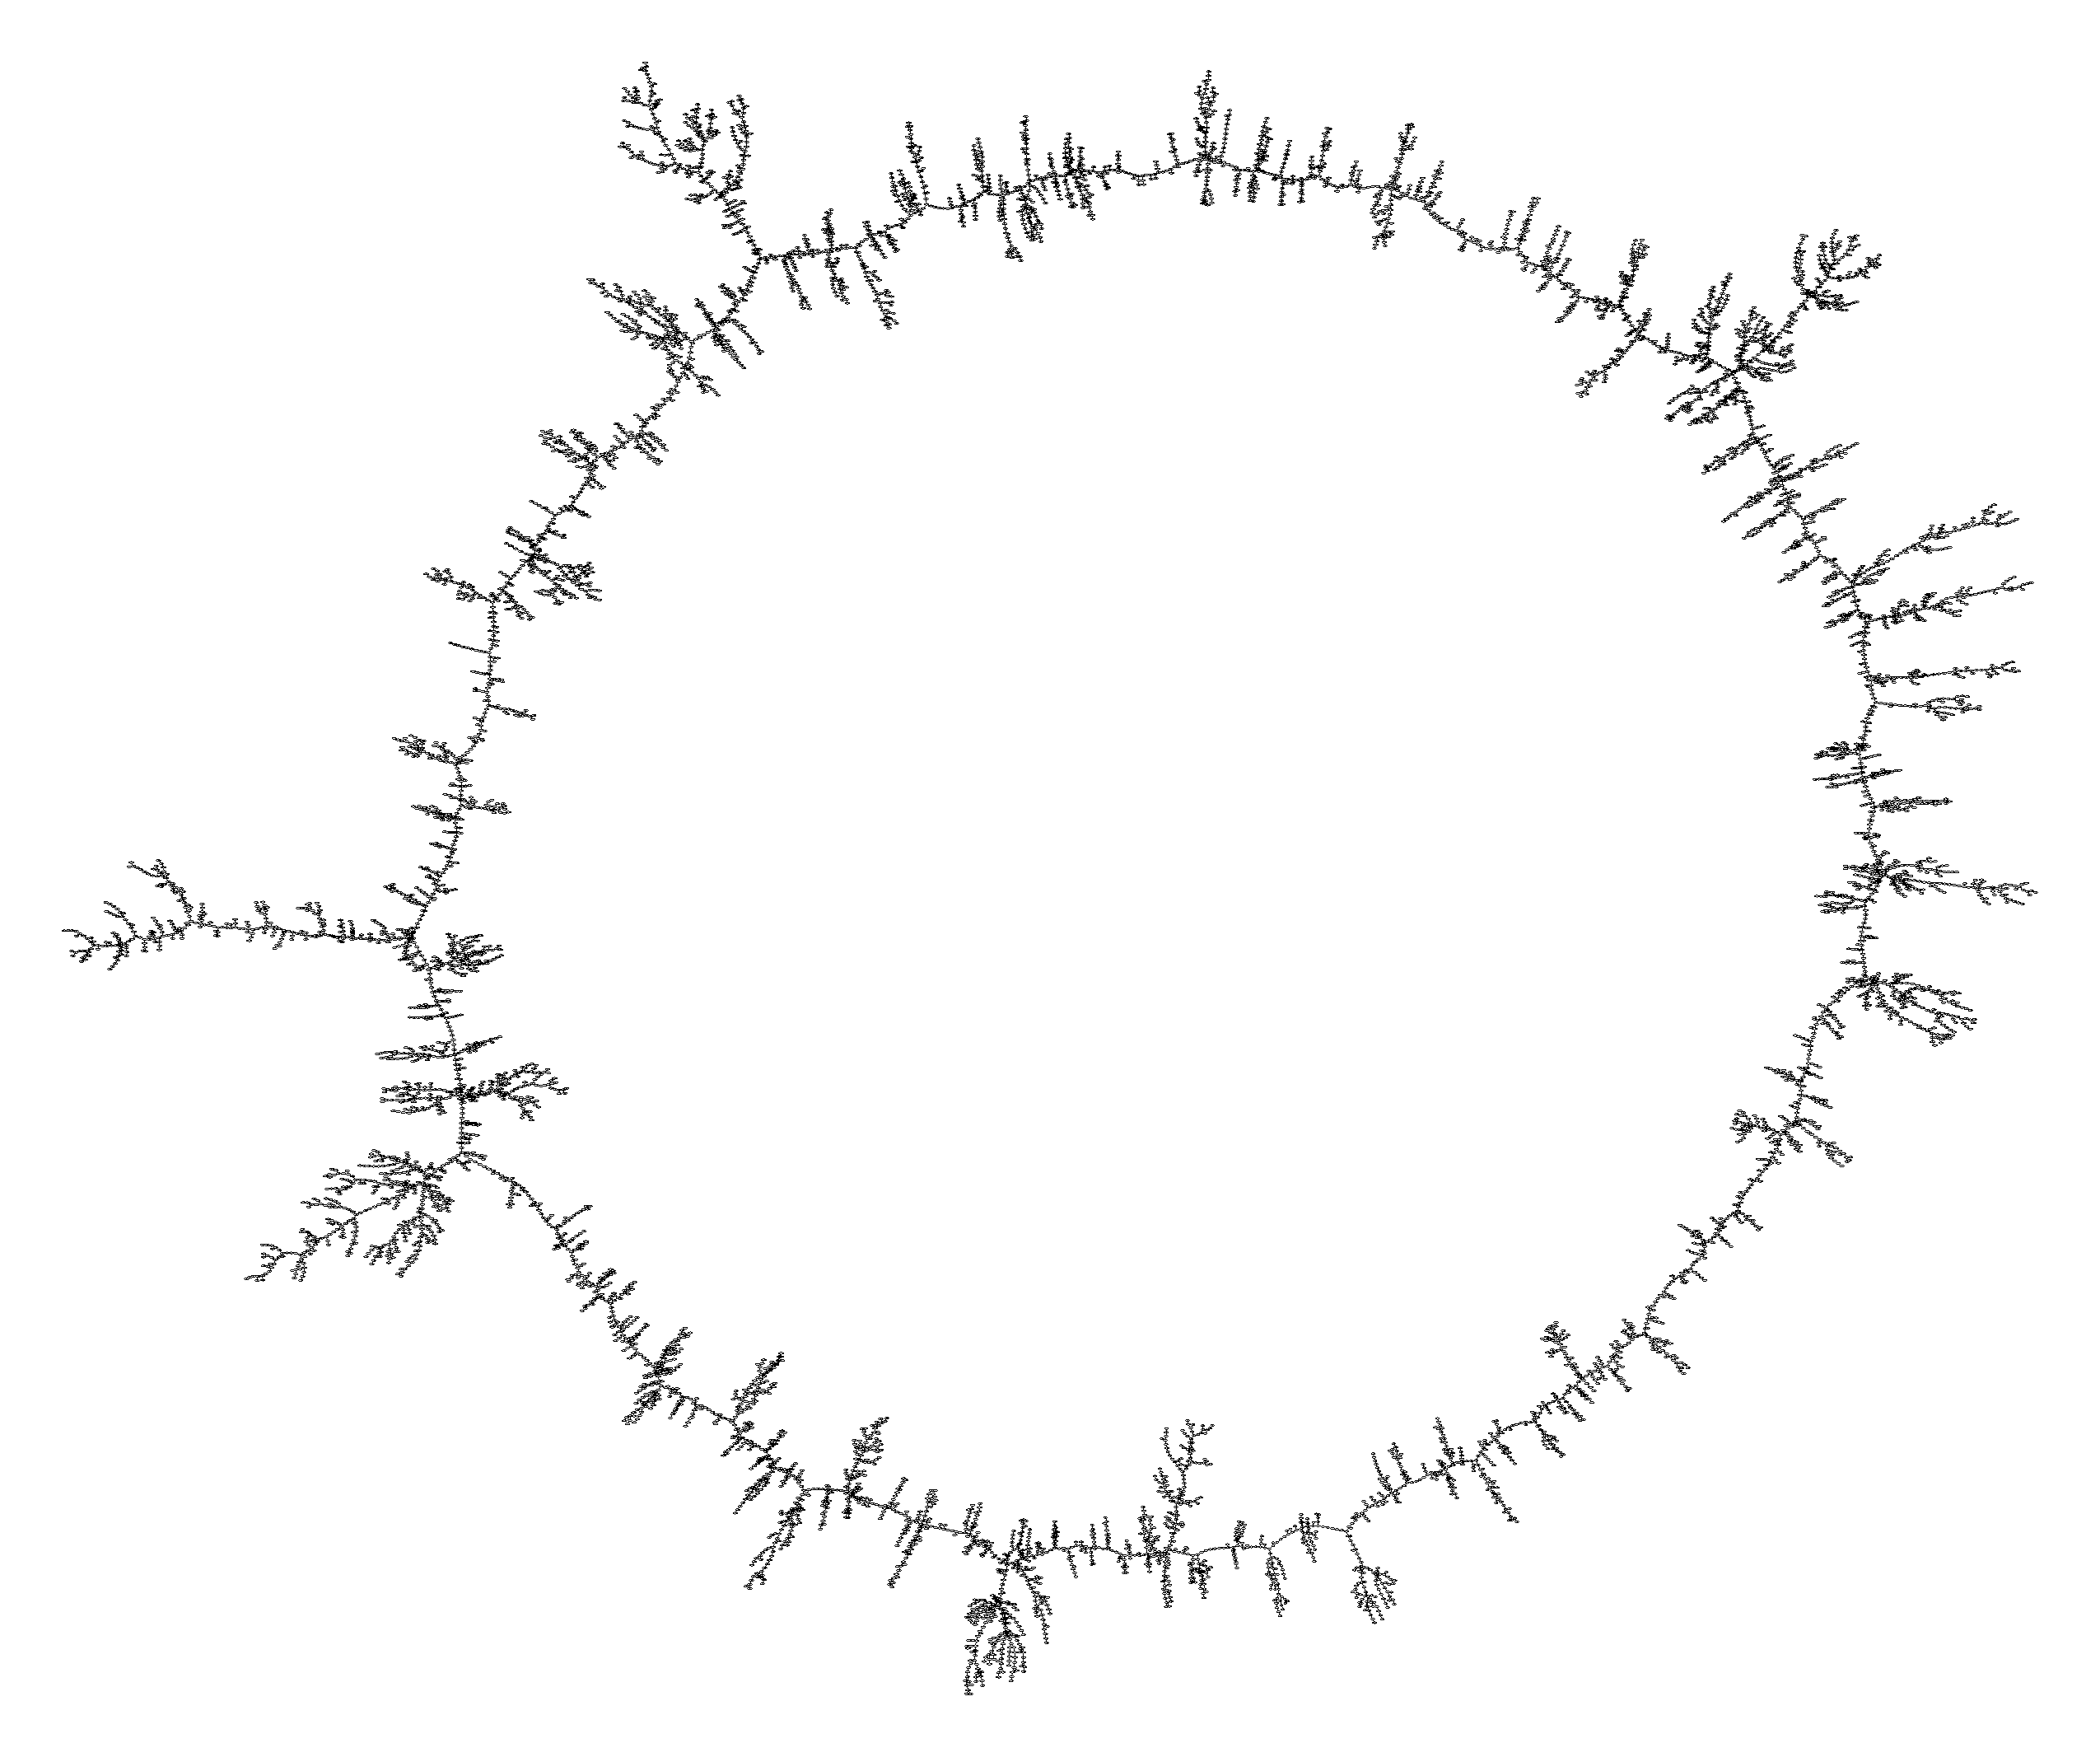
\includegraphics[width=3in]{figures/f3b015}
\caption{Graph visualizations demonstrating the decreasing 
fidelity of graph structure with increasing false positive rate. From 
top left to bottom right, the false positive rates are 0.01, 0.05, 0.10, 
and 0.15.}
\end{figure}

In addition, it is simple to see that a linear increase in the false 
positive rate results in a linear increase in the number of expected 
neighbors for a particular k-mer. For most isolated (i.e. no adjacent 
``real'' k-mers) k-mers, the calculation is 
E(erroneous neighbors)$ = 8 \times p_f$. Thus, the local graph 
structure breaks down in a linear fashion. However, this offers no insight 
to how the global graph structure degrades.
% @JAP if it is the graph you are thinking of, I am not sure that I 
% ever incorporated it into the paper, unless you are thinking of something 
% Arend did. if it is that graph, then I didn't think to include it 
% because the linear effect seems to be intuitive

\subsection{Breakdown In Global Connectivity}
We wanted to explore the point at which our data structure systematically 
engenders false long-range connections, 
so we randomly inserted 31-mers into Bloom
filters with increasing false positive rates and calculated the average
cluster size for each false positive rate. Figure 2 demonstrates that 
the average cluster
size rapidly increases as a specific threshold is approached,
which appears to be at a FP rate near 0.18 for k=31. Beyond 0.18, 
the connected components begin to join together as a single giant 
cluster, and it is no longer possible to distinguish between reads 
that do not overlap in the original dataset using the Bloom filter.

\begin{figure}
\center{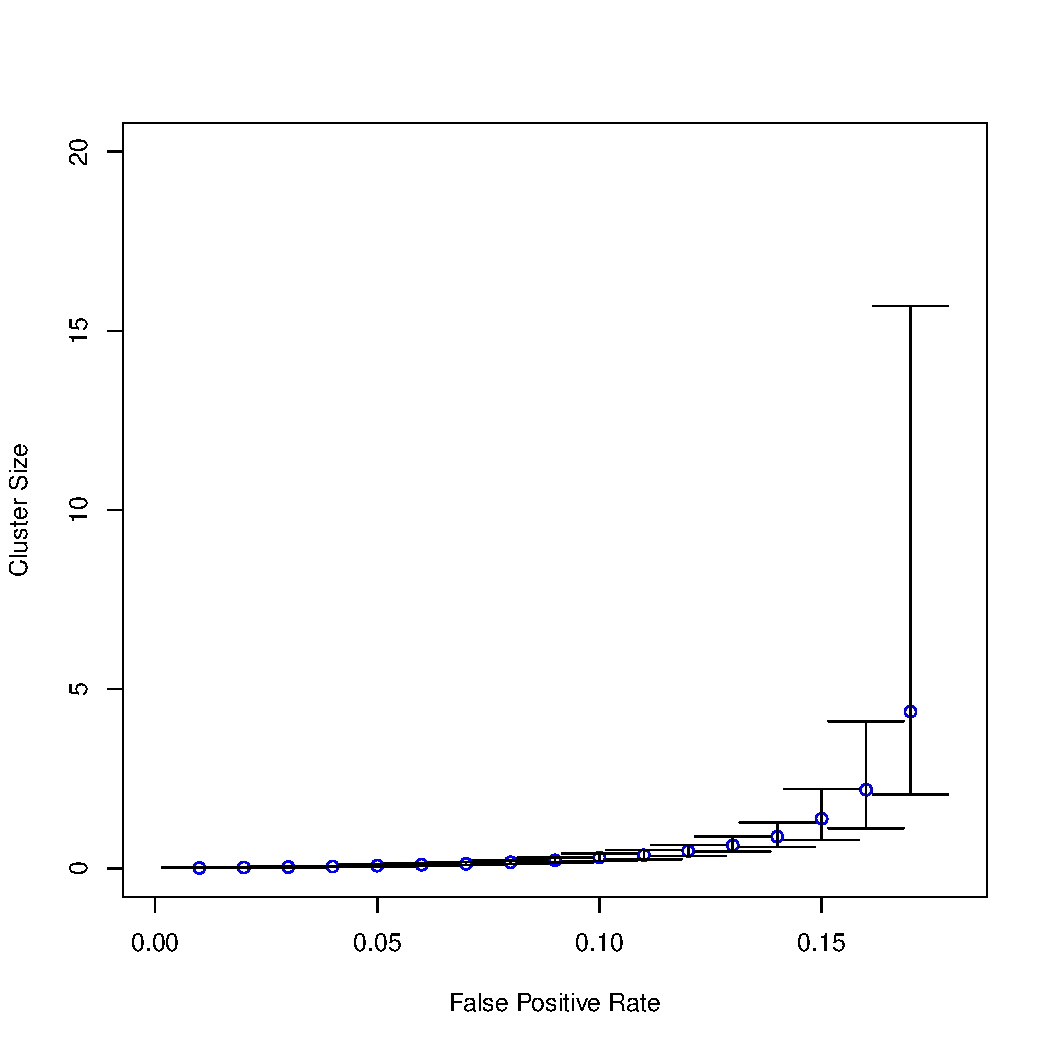
\includegraphics[width=5in]{newclustersize}}
\caption{Average cluster size versus false positive rate. The average 
cluster size sharply increases as the false positive 
rate approaches the percolation threshold.
}
\end{figure}

As the false positive rate increases, there appears to be a sudden
transition from where the graph is comprised of disconnected 
components to where they begin to erroneously connect (Figure 2). 
In contrast to the linear-style change seen 
in local graph structure as the false positive rate increases linearly, 
the change in global graph structure is abrupt as previously disconnected 
clusters join together.  
This rapid change appears to resemble a phase transition, which for graphs
can be 
discussed in terms of percolation theory. We can map 
our problem to site percolation by considering a probability $p$ that a 
particular k-mer is the ``on'' state. This is in contrast to bond percolation where 
$p$ represents the probability of a particular edge being in the ``on'' state. As
long as the false positive rate is below the percolation threshold $p_\theta$ (in
the subcritical phase), it is feasible to traverse the graph. If the
false positive rate is at or above this (in the supercritical phase), then graph
traversal is unpractical.

% @CTB MENTION ITERATIVE PARTITIONING

The percolation thresholds for finite graphs can be estimated by
finding where the cluster size distribution transitions from linear to
quadratic in form (CHECK ME).  Using the calculation method described
in \emph{Methods}, we found that the site percolation threshold for
DNA k-mer graphs is $p_\theta = 0.183 \pm 0.001$.  The percolation
threshold appears to be the same for different $k$, which suggests
that it is independent of $k$. This implies that as long as
the false positive rate is below $0.183$, connected components in the
graph are unlikely to erroneously connect to one another.

\subsection{Large-scale Graph Structure Retained to Percolation Threshold}
The results from cluster size analysis and the percolation threshold 
estimation suggest that 
global connectivity of the graph is unlikely 
to change below the percolation threhold. To demonstrate this, we employed 
the diameter metric in graph theory.  
The diameter of a connected component in a graph is a measure of 
the length of the ``longest shortest'' 
path between any two vertices\cite{bondy2008graph}.
In our case, we only considered paths between two real k-mers
in the dataset for the only component that contains real k-mers. 
We randomly generated 58bp long circular
chromosomes to construct components containing 50 k-mers (setting $k=8$) and 
calculated the diameter at different false positive rates, averaging
the results from multiple runs ($n=20$).
% I had to set k to be low because I wanted to go beyond the percolation
% threshold, and I couldn't think of a straightforward way to handle it
% for a high value of k...n=100 or whatever would be pretty easy...I just 
% wanted to get the graph generated
As Figure 3 shows, 
erroneous connections between pairs of ``real'' k-mers are unlikely
below the 
percolation threshold. At or after the percolation threshold, spurious connections 
between real k-mers are created, which lowers the diameter. 
Thus, the larger scale graph structure is retained until $p=0.183$, as suggested by the cluster size analysis and percolation results.

\begin{figure}
\center{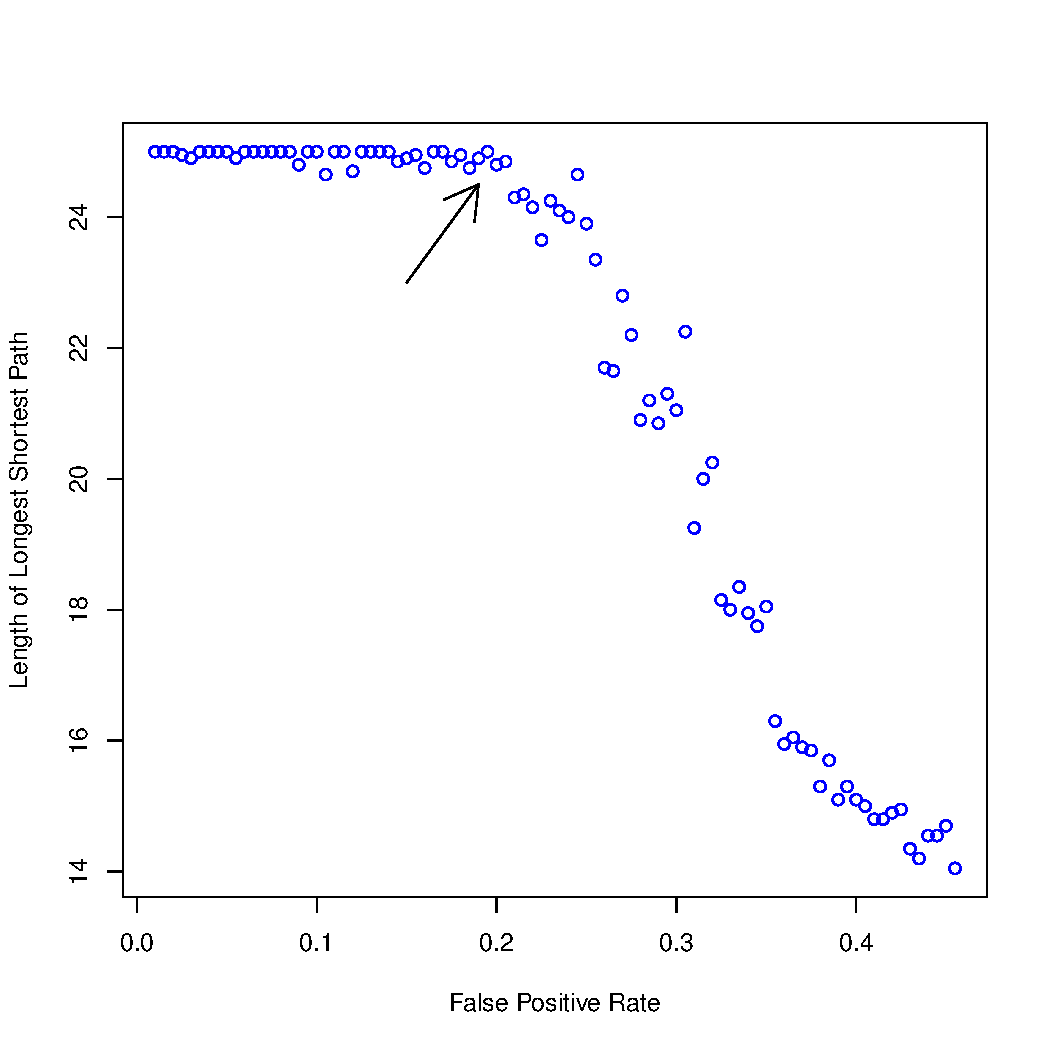
\includegraphics[width=5in]{figures/diameter}}
\caption{Length of Longest Shortest Path by False Positive Rate. The 
length of the longest shortest path of randomly generated 58bp 
long circular chromosomes in 8-mer 
space for different false positive rates. Only real (non-error) k-mers are
considered for starting and ending points.}
\end{figure}

\subsection{Sequencing Errors Eclipse Errors From Graph Representation}
One important consideration when determining the usefulness of our
k-mer graph representation is how it compares to graphs built from
real data from massively parallel sequencers such as Illumina, which
contains base calling errors.  In de Bruijn graph-based assemblers,
sequencing errors add to the graph complexity and make it more
difficult to find high-quality paths for generating long, accurate
contigs. Since our approach generates false positives, we wanted to
compare the error rate from the Bloom filter graph with experimental
errors generated by sequencing. We used an
\emph{E. coli} K-12 MG1665 genome to compare various graph invariants
between an Illumina dataset of the same strain (see \emph{Methods}),
an exact representation of the genome, and inexact representations
with different false positive rates.

\begin{figure}
\begin{tabular}{ | c || c | c | c | c | c | }
\hline
 & No. K-mers & No. Additional & No. Missing & Deg $\ge 2$ & \% Real K-mers \\ \hline \hline
\emph{E. coli} 0 \% & 4,530,123 & 0 & 0 & 50,605 & 100 \\ \hline
\emph{E. coli} 1 \% & 4,814,050 & 283,927 & 0 & 313,844 & 94.1 \\ \hline
\emph{E. coli} 5 \% & 6,349,301 & 1,819,178 & 0 & 1,339,102 & 71.3 \\ \hline
Reads 0 \% & 45,566,033 & 41,036,029 & 119 & 7,700,483 & 9.9 \\ \hline
Reads 1 \% & 48,237,038 & 43,707,032 & 117 & 9,771,028 & 9.4 \\ \hline
Reads 5 \% & 62,094,757 & 57,564,749 & 115 & 18,116,934 & 7.3 \\
\hline
\end{tabular}
\caption{An exact \emph{E. coli} genome representation of 17-mers was compared with 
two inexact ones as well as an exact and two inexact representations of an Illumina 
\emph{E. coli} dataset.
CTB: put in commas in numbers; add 15\%; label first column; add memory usage column.}
\end{figure}

For these comparisons, we used a $k$ value of 17, which allows for exact
representation in memory. We found 
that there were 50,605 17-mers in the exact representation that were no
part of a simple line, i.e. had more 
than two neighbors (degree $>$ 2). As the false positive rate 
increased, the number of these 
17-mers increased in the expected linear fashion in addition to the number of 
false positive 17-mers found in each connected component. Furthermore, the number of 
``real'' 17-mers, those that are not false positives, 
comprise the majority of the graph.

In contrast, when we examined an exact representation of an Illumina
dataset, only 9.9\% of the k-mers in the graph truly exist in the
reference genome. Note that we only counted false positive k-mers that
are transitively connected to least one real k-mer. The
number of 17-mers with more than 2 neighbors is higher
than for the exact representation of the genome, which demonstrates
that sequencing errors add to the complexity of the
graph. Thus, we find that the errors demonstrated by sequencers dwarf
the errors caused by the inexact graph representation below a
reasonable false positive rate.

\subsection{Graph Representation Can Be Used To Partition Sequencing Data}
One advantage to the compressible graph is that it can be used to
separate reads in a dataset to make the DNA sequence assembly less
memory intensive. The diameter results suggest that unconnected
components are unlikely to connect below the percolation threshold. To
show this, we broke up the \emph{E. coli} genome at k-mers with a
degree greater than two and compared it with a simulated dataset of
1,000 randomly generated contigs containing 10,000bp each. Using
$k=32$, we partitioned the datasets using the procedure described in
\emph{Methods} at different false positive rates (Figure 5). As
expected, the resulting number of partitions did not change for the
simulated dataset. For the \emph{E. coli} dataset, the number of
partitions drops slowly with increasing false positives, which is
likely due to components that are close but were forcibly disconnected
in our simulated data set.
% @CTB repartitioning

\begin{figure}
\center{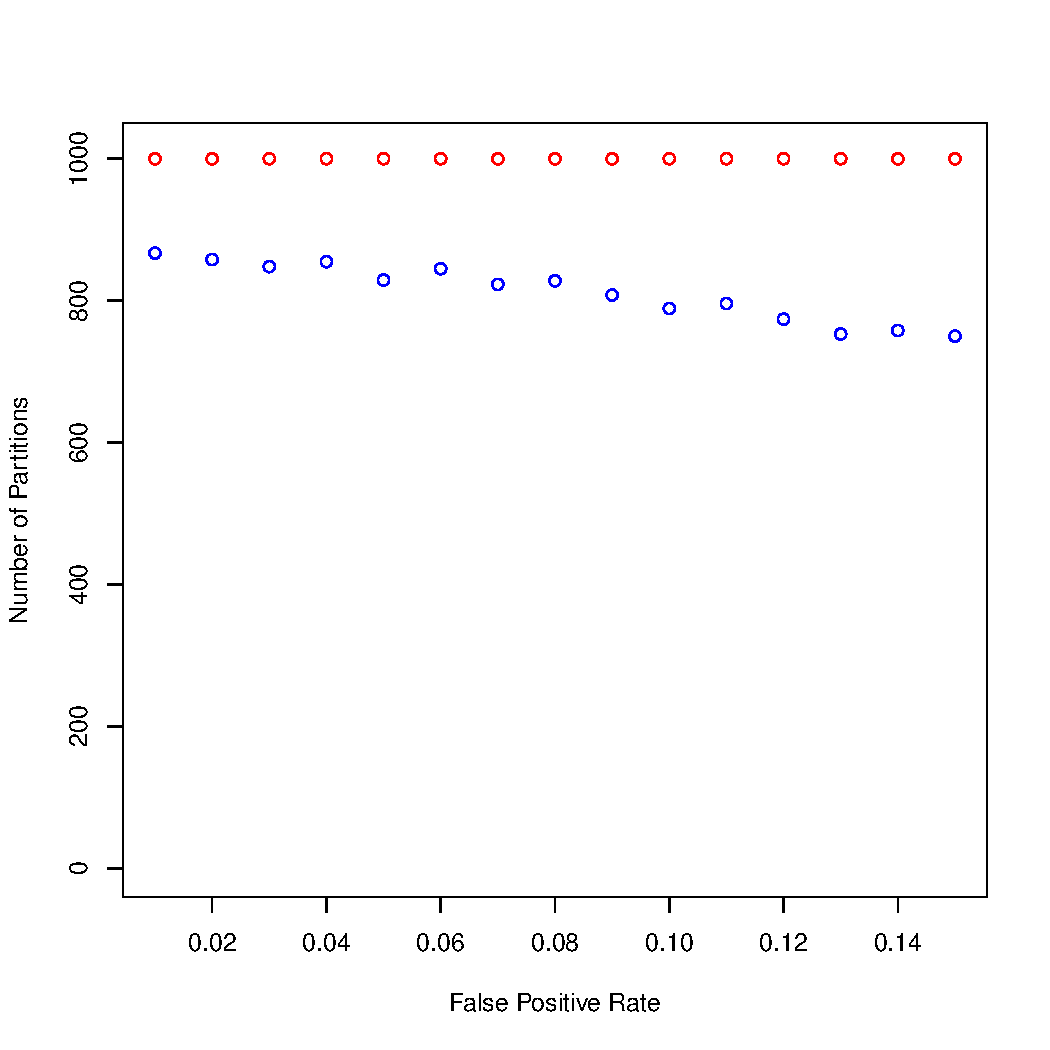
\includegraphics[width=5in]{figures/partplot}}
\caption{Number of Partitions by False Positive Rate. The 
graph shows the resulting number of partitions for the 
\emph{E. coli} genome broken up in high-complexity regions (blue) and 
a simulated dataset with 1,000 contigs of 10,000 bp each (red).}
\end{figure}

\section{Discussion}

\subsection{Bloom Filters Can Be Used To Accurately Store Large Assembly Graphs}
The compressible graph representation we have built on a Bloom filter
is an efficient way to store and traverse k-mer graphs.  Per k-mer
memory usage is low compared to exact approaches without false positives,
and memory usage is independent of k.  K-mer vertex lookup and
local traversal are constant time.  The primary data structure can
also be implemented in constant memory.  This graph representation is
also easy to implement correctly.

The probabilistic nature of the data structure is a significant
concern, but the collision rate and resulting increase in false local
connectivity are predictable.  On a larger scale, we can link the
rate of increase in global connectivity from false positives to a
first-order phase transition, which lets us define a broad range of
parameters for which the global graph structure is extremely accurate.
Within this range, the primary effect of decreasing memory is to increase
traversal computation.  Note that this also provides a systematic way
to trade time spent in traversal (computation) off against memory. As shown 
in Figure 2, the amount of traversal from each k-mer increases 
(affecting computation) as the false positive rate increases, which 
is determined by the amount of memory that is allocated to the data 
structure.

The effect of increasing false positive rate as ``error'' can be
compared to the effect of sequencing errors.  Sequencing error
introduces both false negatives (by eliminating ``true'' k-mers from
low coverage samples) and false positives.  Novel k-mers
from sequencing errors also often result in k-mers that are
a low Hamming distance from the true k-mer, which can result in
elaborate graph structures.  In contrast, the Bloom graph error is
entirely one-sided, only resulting in false positives; moreover, these
false positives are uncorrelated with the ``true'' k-mers from which
they arise, and generally contribute to local graph structure only 
in a linear fashion as the false positive rate increases.

Overall, the Bloom k-mer graph is an efficient data structure for
storing and traversing large k-mer graphs.

\subsection{Decomposing Large Graphs}
Figure 5 shows that we can partition
genome connectivity graphs into perfectly disconnected subcomponents
given suitably chosen breakpoints.  Combined with the scaling
properties of the graph representation, this offers a way to
efficiently apply a "divide and conquer" strategy to assembly
problems.  The next challenge is to develop an efficient way for
finding breakpoints, or equivalently to characterize minimally
connected components; existing graph algorithms for e.g. "betweenness
centrality" do not scale to graphs with millions or billions of nodes.

While the assembly graph is entirely connected for most genomes --
either because there is a single chromosome, or because of repeat
elements that connect chromosomes -- we note that there are several
biological problems well suited to partitioning.  Both transcriptome
and metagenome sequencing target *populations* of disconnected
sequences.  Trinity, for example, relies on a partitioning approach in
the second phase (XXX) of transcriptome assembly; and both meta-idb
and metavelvet rely on locality of connections for metagenome
assembly.  However, these approaches do not address scaling.

\subsection{Other Uses}

There are many potential uses for a scalable de Bruijn graph representation.

Small component elimination.

Repeat structure characterization and filtering.

Graph search.

Graph-based error correction.

\subsection{Applying Bloom K-mer Graphs To DNA Sequence Assembly}
Bloom k-mer graphs may not be directly useful for traditional
approaches to DNA assembly, which rely on systematic heuristic
transformations of graph structure to find an optimal path through the
graph.  This is because the Bloom graph, as presented here, is limited
to representing k-mer graphs for a fixed k, and paths cannot readily
be compacted or eliminated.
% @CTB What did I mean ``for a fixed k''?  I don't know of any DBG
% reps that don't use a fixed k!

There are many uses, however, for an extremely scalable
graph representation.  Below we discuss the use of the
Bloom k-mer graph data structure as a vehicle for exploring graph
properties and filtering data sets.

For low-coverage samples, assembly graphs may contain many small
unconnected components, that represent unconnected sequences.
% @CTB why?  Beacuse of low coverage! Reiterate I guess.
Sequences contributing to these unconnected components can be safely
eliminated from the originating data sets without affecting the final
assembly.  This can be done efficiently with a simple limited depth
graph search algorithm. Since connected components in the graph 
are unlikely to erroneously connect when the false positive rate 
is below the percolation threshold, graph traversal is only affected 
by the minor changes to the local graph structure.

More generally, assembly graphs may contain many disconnected
subgraphs, due to the structure of the source data (e.g. transcriptome
or metagenome sequencing) or because of low coverage.  These subgraphs
can safely be partitioned into separate graphs without affecting the
final assembly, reducing the memory and computation required for
assembly of the whole to that required for the largest subgraph.
% @CTB discuss local vs global structure changes from FP on this.

The Bloom k-mer graph can also be used to do de novo repeat discovery
in collections of unassembled reads.  This in turn can be applied to
filtering of repeats prior to assembly\cite{hydra}, or for isolating
repeats from shallow or exploratory sequencing efforts.

It may also be possible to adapt sequence structure (e.g. ORF),
homology (BLAST), and domain search (HMMER) algorithms to search this
graph structure instead of searching either unassembled reads or
assemblies (Fish, Brown and Cole, pers communication).  Because 
assembly graphs implicitly collapse identical
sequences into a single path, this may be a more scalable approach to
targetted-gene analysis for metagenomics than current approaches
(which rely on searching individual reads that may be overlapping or identical).  Also note that, unlike
sequencing errors, the false positives in the Bloom graph will
generally bear no resemblance to biologically valid matches, which 
makes their detection during graph traversal easier.

The Bloom k-mer graph could also be used to develop connectivity-based
read trimming and correction algorithms.  For example, low-abundance
reads that contribute to ``spurs'' or ``sidings'' in otherwise
high-coverage regions could be corrected to match the
consensus, or trimmed to eliminate the divergent sequence.

One particularly intriguing option is to use the memory-efficient and
scalable Bloom k-mer graph representation as a component of a hybrid
assembler.  The k-mer graph approach could be used to identify
reads that belong to high-complexity regions, and extract them for
later resolution with more targetted approaches, e.g. an OLC assembler.
Alternatively, regions could be locally examined and extracted for
assembly, and then passed to scaffolding toolkit like Bambus for 
larger-scale connectivity\cite{bambus}.

\subsection{Dramatic Scaling}
It is clear that sequencing capacity will continue to outpace Moore's 
law and new methods must address this. Our graph representation allows 
for excellent scaling capabilities at the cost of a manageable false positive rate. 
As mentioned previously, $\sim 6.22$ bits per k-mer are required for a 
false positve rate of 5\%, so that modern computers with 
over 512GB of memory can handle graphs containing hundreds of billions of k-mers.

Another consideration is that assembly is generally difficult to parallelize. 
ABySS and Contrail (citation?), for example, place different parts of the 
graph on separate nodes. However, this can hinder performance due to 
network latency. Having the ability to examine the entire graph in memory 
before distributing the graph across multiple processors can minimize the
degree to which processors need to query one another. A smaller memory 
footprint can also mean that the entire assembly could be performed on 
a single node, if computational resources are limited.

Finally, though so-called ``third-generation'' sequencers are showing promise with 
longer reads and better error rates, we believe that improvements in these 
areas will not solve the scaling issue in certain domains. In particular, 
mRNAseq and metagenomics datasets are still sensitive to sampling depth as
well as read length. Differential expression detection and assembly 
of low-expressed genes are difficult without deep coverage. Thus
the required coverage level for an mRNAseq dataset is high, leading to large
data sets. Furthermore, many environmental samples with 
diverse microbial communities are estimated to require several terabases of sequencing 
in order to achieve a modest coverage level (citation?  my refs CTB). In both of these domains, better 
scaling algorithms are needed to handle these complex assemblies. 

\subsection{Concluding Remarks}
We have shown that representing a k-mer graph on a Bloom filter-like data 
structure can create an inexact, yet lightweight graph representation of 
a k-mer graph. This inexactness can be precisely known based on the occupancy 
of each hash table, and we demonstrated that our approach is still useful 
below a specific false positive rate. We conclude that while this representation 
may not be ideal for a final assembly, it can be useful for pre-filtering 
strategies and solving the scaling and memory bottleneck problems that we 
currently face in sequence assembly.

\subsection{Acknowledgements}

Jim Cole and Jordan Fish.  Qingpeng.  Adina.  Adami.  JGI folk.

\bibliographystyle{abbrv}
\bibliography{kmer-percolation}
\end{document}


